\documentclass[12pt]{article}
\usepackage[top=1in, bottom=1in, left=.75in, right=.75in]{geometry}
\usepackage{amsmath, enumerate}
\usepackage{fancyhdr}
\usepackage{graphicx, xcolor, setspace, array}
\usepackage{txfonts}
\usepackage{multicol,coordsys,pgfplots}
% \usepackage{enumitem}
\usepackage[scaled=0.86]{helvet}
\renewcommand{\emph}[1]{\textsf{\textbf{#1}}}
\usepackage{anyfontsize}
% \usepackage{times}
% \usepackage[lf]{MinionPro}
\usepackage{tikz,pgfplots}
%\def\degC{{}^\circ{\rm C}}
\def\ra{\rightarrow}
\usetikzlibrary{calc,arrows.meta}
\pgfplotsset{compat = newest}
\newcommand{\blank}[1]{\rule{#1}{0.75pt}}

\pgfplotsset{my style/.append style={axis x line=middle, axis y line=
middle, xlabel={$x$}, ylabel={$y$}}}

%axis equal

%yticklabels={,,} , xticklabels={,,}

% \setmainfont{Times}
% \def\sansfont{Lucida Grande Bold}
\parindent 0pt
\parskip 4pt
\pagestyle{fancy}
\fancyfoot[C]{\emph{\thepage}}
\fancyfoot[R]{v3} %%%%%% <-- Version Info
\fancyhead[L]{\ifnum \value{page} > 1\relax\emph{Math F113X: Exam 1}\fi}
\fancyhead[R]{\ifnum \value{page} > 1\relax\emph{Fall 2025}\fi}
\headheight 15pt
\renewcommand{\headrulewidth}{0pt}
\renewcommand{\footrulewidth}{0pt}
\let\ds\displaystyle
\def\continued{{\emph {Continued....}}}
\def\continuing{{\emph {Problem \arabic{probcount} continued....}}\par\vskip 4pt}


\newcounter{probcount}
\newcounter{subprobcount}
\newcommand{\thesubproblem}{\emph{\alph{subprobcount}.}}
\def\problem#1{\setcounter{subprobcount}{0}%
\addtocounter{probcount}{1}{\emph{\arabic{probcount}.\hskip 1em(#1)}}\par}
\def\subproblem#1{\par\hangindent=1em\hangafter=0{%
\addtocounter{subprobcount}{1}\thesubproblem\emph{#1}\hskip 1em}}
\def\probskip{\vskip 10pt}
\def\medprobskip{\vskip 2in}
\def\subprobskip{\vskip 45pt}
\def\bigprobskip{\vskip 4in}


\newenvironment{subproblems}{%
\begin{enumerate}%
\setcounter{enumi}{\value{subprobcount}}%
\renewcommand{\theenumi}{\emph{\alph{enumi}}}}%
{\setcounter{subprobcount}{\value{enumi}}\end{enumerate}}


\newcommand{\be}{\begin{enumerate}}
\newcommand{\ee}{\end{enumerate}}


\newcommand{\ans}[1][1in]{\rule{#1}{.5pt}}



\begin{document}

{\emph{\fontsize{26}{28}\selectfont Fall 2025 \hfill
%{\fontsize{32}{36}\selectfont Calculus 1: Midterm 1}
\hfill Math F113X}}

\begin{center}
{\emph{%\fontsize{26}{28}\selectfont Spring 2024 
%%\hfill
{\fontsize{32}{36}\selectfont Exam 1}
%%\hfill Math F251X}
}}
\end{center}

%\vskip 2cm
\strut\vtop{\halign{\emph#\hskip 0.5em\hfil&#\hbox to 2in{\hrulefill}\cr
\emph{\fontsize{18}{22}\selectfont Name:}&\cr
%\noalign{\vskip 10pt}
%\emph{\fontsize{18}{22}\selectfont Student Id:}&\cr
%\noalign{\vskip 10pt}
%\emph{\fontsize{18}{22}\selectfont Calculator Model:}&\cr
}}
\hfill
\vtop{\halign{\emph{\fontsize{18}{22}\selectfont #}\hfil& \emph{\fontsize{18}{22}\selectfont\hskip 0.5ex $\square$ #}\hfil\cr
Section: & 10:30 am (Leah Berman)\cr
\noalign{\vskip 4pt}
         & 11:45 am (Kevin Meek)\cr
         \noalign{\vskip 4pt}
          & online (Kevin Meek)\cr
}}

\vfill
{\fontsize{18}{22}\selectfont\emph{Rules:}}

\begin{itemize}
\item Partial credit will be awarded, but you must show your work.

\item You may have 1/2 of a standard page of paper ($8.5''\times 5.5''$ or $11''\times 4.25''$)  of notes, both sides.

\item Calculators are allowed. 

\item Place a box around your  \fbox{FINAL ANSWER} to each question where appropriate.

\item Turn off anything that might go beep during the exam.

\end{itemize}

%If you need extra space, you can use the back sides of the pages.
%Please make it obvious  when you have done so.



Good luck!

\vfill
\def\emptybox{\hbox to 2em{\vrule height 16pt depth 8pt width 0pt\hfil}}
\def\tline{\noalign{\hrule}}
\centerline{\vbox{\offinterlineskip
{
\bf\sf\fontsize{18pt}{22pt}\selectfont
\hrule
\halign{
\vrule#&\strut\quad\hfil#\hfil\quad&\vrule#&\quad\hfil#\hfil\quad
&\vrule#&\quad\hfil#\hfil\quad&\vrule#\cr
height 3pt&\omit&&\omit&&\omit&\cr
&Problem&&Possible&&Score&\cr\tline
height 3pt&\omit&&\omit&&\omit&\cr
&1&&20 &&\emptybox&\cr\tline
&2&&12	&&\emptybox&\cr\tline
&3&&20	&&\emptybox&\cr\tline
&4&&12	&&\emptybox&\cr\tline
&5&&18	&&\emptybox&\cr\tline
&6&&18	&&\emptybox&\cr\tline
%&7&&	&&\emptybox&\cr\tline
%&8&&	&&\emptybox&\cr\tline
%&9&&	&&\emptybox&\cr\tline \tline
&Extra Credit&&(6)&&\emptybox&\cr\tline
&Total&&100&&\emptybox&\cr
}\hrule}}}

\newpage

%%Problem 1

%%RCV
\problem{20 points} 

A certain borough in Alaska has switched to using \emph{Instant Runoff Voting (Ranked Choice Voting) }to determine the winner of its mayoral races.

In a recent municipal election, the preference schedule for the race was as follows:

\begin{center}

\begin{tabular}{|l || c | c | c | c | c| c|}
\hline
& 45& 40& 35& 15& 10&5\\ \hline
%&Hopkins& Kassel & Sampson & Ward \\
1st choice & Bork & Alton & Clay & Bork & Davis & Davis\\
2nd choice & Alton & Davis & Alton & Clay & Clay& Clay\\
3rd choice & Clay & Clay & Bork & Davis & Bork & Alton\\
4th choice & Davis & Bork & Davis & Alton & Alton & Bork\\
\hline
\end{tabular}

\end{center}

\begin{subproblems}
\item How many voters voted in the election?  \ans %\ Provide your computation.

\vspace{.25in}

\item How many voters are needed to have a majority of the votes? \ans

\vspace{.25in}

\item Was there a winner after round 1 (that is, before anyone was eliminated)? Why or why not? Explain your answer.

\vspace{.5in}

\item Was anyone eliminated in round 1?  Explain your answer.

\vspace{.5in}

\item Determine the winner of the election. Show your work clearly, in a way that someone else can follow. If you require multiple rounds, show the computations clearly, and clearly state which candidate is eliminated.

\vfill


The winner of the election was \ans\ after \ans\ rounds.
\end{subproblems}
\newpage


%%%%%%%%%%%%%%%%%

%%Problem 2
%% VArious voting questions
%%%%%%%%%%%%%%%%%%%%%%%%%%%%%%



\problem{12 points}  Students in a dorm are voting on which Halloween activity  the dorm should put on for local children. They are choosing among four choices, here conveniently labeled A, B, C, D. The preference schedule is below. 

%45	15	15	10
%A	B	D	D
%D	D	C	B
%B	A	B	A
%C	C	A	C

\begin{tabular}{|c|| c|c|c|c|}
\hline
number of voters&45&15&15&10\\
\hline \hline
1st choice&A	&B	&D	&D\\ \hline
2nd choice&D	&D	&C	&B\\ \hline
3rd choice&B	&A	&B	&A\\ \hline
4th choice&C	&C	&A	&C\\ \hline
\end{tabular}


	\begin{subproblems}
	\item  How many voters participated? \ans \\
          \vspace{0.2cm}

          \item Who was the plurality winner? \ans \\
            \vspace{0.2cm}
	
	\item Find the winner under the Borda Count Method. (You must clearly show your calculations.)
	
	\vfill
	\vfill
	
	
	\item  Pick a fairness criterion that is violated in this election and provide a short explanation with supporting computation explaining why it is violated. Mark the box of the criterion that is violated.
	
$\Box \quad$	Condorcet Criterion\\
$\Box \quad$	Monotonicity Criterion\\
$\Box \quad$	Majority Criterion\\
$\Box \quad$	Independence of Irrelevant Alternatives (IIA) Criterion\\
\vspace{0.2cm}
	
\item Explain how you know this criterion is violated.
	\vfill
	
	
	
		\end{subproblems}		
		
		
\newpage
%Problem 3
%weighted voting problem 2

\problem{20 points} 
\begin{subproblems}
\item In the weighted voting system $[q:10,8,2,1]$, what is the {\bf
    largest} value $q$ can take? Justify your answer with a
  calculation.
  \vfill
\item In the weighted voting system $[q:25,7,6,3]$, find a value for
  $q$ so that $P_1$ is a dictator. Justify your answer with a
  calculation.
  \vfill
\item Consider the weighted voting system [26:10,8,6,4,4,2,1].
  \be[i.]
  \item Identify any players with veto power or state that none
    exist. Justify your answer.\\
    \vfill
  \item Explain why $P_6$, who has 2 votes, is not a dummy. \\
    \vfill
    \ee
\end{subproblems}
\newpage




%%%%%%%%%%%%%%%%%%%%%
%%%vBahnzaf

\problem{12 points} 
Consider the weighted voting system $[20:12,10,5,3]$
	\begin{subproblems}
\item Find all winning coalitions. 

\underline{Winning Coalitions}

\vfill

\vfill

\item Underline critical players in your winning coalitions above.
\item Fill in the following chart:

\bigskip

\begin{tabular}{ c | p{1in}  | c}
Player & & Banzhaf Power Index\\ \hline
$P_{1}$ && \\[12 pt] \hline
$P_{2}$ && \\[12 pt] \hline
$P_{3}$ && \\[12 pt] \hline
$P_{4}$ && \\[12 pt]

\end{tabular}

	\end{subproblems}
	\vfill

\newpage
%%%%%%%%%%%%%%%%%%%
%%Divider-chooser

\problem{18 points}

Suci and Matilda are dividing an  ice cream cake with two flavors: hazelnut and chocolate. Each flavor takes up the same amount of cake, and the total value of the cake is \$32.

\newcommand{\cake}{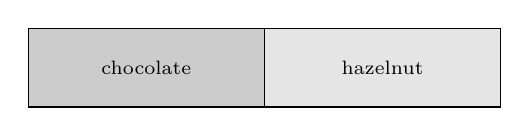
\begin{tikzpicture}[scale = .5]
\draw[fill = gray!40] (0,0) rectangle (6,2);
\node[font = \scriptsize] at (3,1) {chocolate};
\draw[fill = gray!20] (6,0) rectangle (12,2);
\node[font = \scriptsize] at (6+3,1) {hazelnut};
\end{tikzpicture}
}

\begin{center}
\cake
\end{center}

\begin{subproblems}
\item What is a fair share of the cake? \ans
\item Suppose

\begin{itemize}
\item Suci likes hazelnut three times as much as chocolate. 
\item Matilda's valuation is listed in the table.
\end{itemize}

 Fill in the table of values for Suci.

\vspace{1cm}

\begin{center}
\begin{tabular}{| c || c | c || c |}
\hline
Person & Chocolate & Hazelnut   & total value\\ \hline
Suci & && \\[12 pt] \hline
Matilda  & 28& 4 &\\[12 pt] \hline
\end{tabular}
\end{center}

\item Suppose Suci is the divider. They divide the cake into two portions: one portion consists of all of the chocolate and 1/3 of the hazelnut, and the other portion consists of the remaining 2/3 of the hazelnut.

%\begin{tabular}{c c}

\begin{center}
\begin{tikzpicture}[scale = .5]
\draw[fill = gray!40] (0,0) rectangle (6,2);
\node[font = \scriptsize] at (3,1) {chocolate};
\draw[fill = gray!20] (6,0) rectangle (6 + 6/3,2);
\node[font = \scriptsize, inner sep = 1 pt] (lbl1) at (6 + 6/6,-1) {$\frac{1}{3}$ hazelnut};
\draw (lbl1) -- (6 + 6/6,1);
\path (4, 2) node[above]{Portion 1};
%
%\begin{scope}[xshift = 1 cm]
%\draw[fill = gray!20] (6+6/3,0) rectangle (12,2);
%\node[font = \scriptsize, inner sep = 1 pt] (lbl2) at (6 + 6/3 + 6/6,-1) {$\frac{2}{3}$ hazelnut};
%\draw (lbl1) -- (6 + 6/3 + 6/6,1);
%\end{scope}
%\end{tikzpicture}
%&
%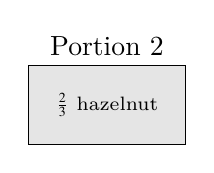
\begin{tikzpicture}[scale = .5]

\begin{scope}[xshift = 3 cm]
\draw[fill = gray!20] (6+6/3,0) rectangle (12,2);
\node[font = \scriptsize] at (10, 1) {$\frac{2}{3}$ hazelnut};
\path (10, 2) node[above]{Portion 2};
\end{scope}
\end{tikzpicture}
\end{center}

%\end{tabular}

\be[i.]
\item Why is that division a fair division for Suci? Provide supporting calculations.


\vfill


\item Which portion of the cake does Matilda choose? Why? Provide supporting calculations.

\vfill
\ee

\end{subproblems}

\newpage

%%%%%%%%%%%%%%%%%%%%%%%%%%%%%%


%
%%%%%%%%%%%%%%%%%%%%%%%
\problem{18 points} %% Lone Divider

\begin{subproblems}
\item Four investors are dividing a piece of land valued at \$320,000. One was chosen as the divider, and their values of the division (in thousands) are shown below. They decide to use the Lone Divider process to divide the land.

\begin{center}

\begin{tabular}{l|| l| l| l| l}
Person & Piece 1 & Piece 2 & Piece 3 & Piece 4\\ \hline
Sonya & \$90 & \$70 & \$ 80 &\$80\\
Cesar & \$80 & \$80 & \$ 80 & \$80 \\
Adrianna & \$60 & \$70 & \$100 & \$90 \\
Raquel & \$70 & \$50 & \$90 & \$110
\end{tabular}

\end{center}

\be[i.]

\item What is the value of a fair share to each investor? \hrulefill

\bigskip

\item Who was the divider? Why? \hrulefill

\bigskip

\item Circle the bids in the table that are fair shares to each investor.

\item Is it possible to allocate the land so that everyone gets a fair share? If so, say who gets which piece of land; if not, say what happens next in the Lone Divider process.
\vspace{1in}

  \ee

\item Suppose three friends are dividing a cake that has been partitioned into three slices. They value the slices as follows:

\begin{center}
\begin{tabular}{l | l l l}
 & Slice 1 & Slice 2 & Slice 3 \\ \hline
 Paul & \$2 & \$1 & \$6 \\
 Quentin & \$3 & \$3 & \$3 \\
 Rosie & \$1.50 & \$2.50 & \$5
\end{tabular}
\end{center}

\be[i.]
\item Circle a fair share for each person.

\item Explain why it's not possible to allocate one slice to each person at the first step.

\vfill

\item Explain what happens next in the Lone-Divider process.


\vfill 
\ee
\end{subproblems}
 

\newpage
%%%%%%%%%%%%%%%%%%%%%%%%%%%

%\fbox{Extra Credit} 
%% Sealed Bids

\emph{Extra Credit} (6 points)

Paula and John, and Willie are dividing up two items: a life-sized replica of Danny DeVito, and a live goat. They submit the following sealed bids for the three items.

\begin{tabular}{| c | c | c || l  |}\hline
& Danny Devito & Goat & total bid  \\ \hline \hline
Paula & \$130 & \$230 & \\ \hline
John & \$260 & \$190  &\\ \hline
Willie & \$310 & \$170 & \\ \hline
\end{tabular}


%\newpage

\be[a.]
\item Determine each person's fair share (in dollars).

\begin{tabular}{c|c|c}
Paula's fair share & John's fair share & Willie's fair share\\
\hline
&&\\
&&\\
&&\\
\end{tabular}

\item  Determine which person gets each item.\\

\begin{tabular}{c|c}
Danny DeVito&Goat\\
\hline
&\\
&\\
\end{tabular}
\item Determine the \textbf{surplus}. Show your work!

\vfill
\vfill

\vfill
\vfill
\item What is the final allocation? Include items and how much each
  person pays and receives in the end? Show your work!

Paula:
\vfill

John:
\vfill

Willie:
\vfill

\ee

%Determine the outcome of the sealed bids process. For each person, list which items they received and whether they got or owed money from the process. Show your work.
%\vfill

%\end{enumerate}

%\end{enumerate}
\end{document}

%%%%ENDDOCUMENT



%%% Local Variables:
%%% mode: LaTeX
%%% TeX-master: t
%%% End:
